\documentclass[12pt,a4paper]{book}
\usepackage[utf8]{inputenc}
\usepackage[english]{babel}
\usepackage{amsmath}
\usepackage{amsfonts}
\usepackage{amssymb}
\usepackage{latexsym}
\usepackage{makeidx}
\usepackage{graphicx}
\usepackage{graphics}
\usepackage{lmodern}
\usepackage{hyperref}
\usepackage{subcaption}
\usepackage{pgfplots}
\usepackage{dsfont}
\usepackage{multicol}
\usepackage{xcolor}
\usepackage{booktabs}
\usepackage{float}
\usepackage{subcaption}
\pgfplotsset{width=10cm,compat=1.9}
\usepgfplotslibrary{external}


\setlength{\parindent}{15px}
\usepackage[left=2cm,right=2cm,top=4cm,bottom=2cm]{geometry}

\author{Daniel Vázquez Lago}
\title{Apuntes Mecánica Clásica II}


\newcommand{\parentesis}[1]{\left( #1  \right)}
\newcommand{\parciales}[2]{\frac{\partial #1}{\partial #2}}
\newcommand{\pparciales}[2]{\parentesis{\parciales{#1}{#2}}}
\newcommand{\ccorchetes}[1]{\left[ #1  \right]}
\newcommand{\D}{\mathrm{d}}
\newcommand{\derivadas}[2]{\frac{\D #1}{\D #2}}
\newcommand{\sech}{\mathrm{sech} \ }
\newcommand{\csch}{\mathrm{csch} \ }
\newcommand{\cotanh}{\mathrm{cotanh}}
\newcommand{\cotan}{\ \mathrm{cotan}}
\newcommand{\Res}{\mathrm{Res}}
\newcommand{\Arg}{\mathrm{arg}}


\newtheorem{theorem}{Teorema}[section]
\newtheorem{corollary}{Corolario}[theorem]
\newtheorem{lemma}{Lema}[section]
\newtheorem{ejemplo}{Ejemplo}[section]


\begin{document}

\maketitle

\newpage

\tableofcontents

\newpage

\chapter{Fuerzas centrales}

\section{Colisiones. Secciones eficaces}

Los experimentos de colisiones son extremadamente importantes para la física, sobretodo para la física cuántica. Los experimentos de \textit{scattering} (colisiones o dispersión) permiten obtener información de una colisión entre dos partículas u objetos a partir de dos el ángulo con el que sale el objeto tras la colisión (o los objetos) y el parámetro de impacto, que es una especie de medida de la puntería, aunque realmente no es así. Definiendolos de manera rigurosa:

\begin{itemize}
\item  \textbf{Ángulo de dispersión:} es el ángulo que forma la dirección que entra y la dirección que sale del objeto estudiado. Se denota por $\theta$.
\item \textbf{Parámetro de impacto:} es la distancia perpendicular entre los objetos que colisionan.
\end{itemize}

En general los problemas de scattering tratan de calcular la relación entre $\theta$ y $b$, calculando $b(\theta)$ o $\theta(b)$. 

\subsection{Sección eficaz de colisión}

Definimos sección eficaz como el área efectiva a partir la cual los objetos interactuen.
Sea $A$ el área total del conjunto de partículas que están quietas (las que reciben el objeto que colisiona), y $n_b$ el número de estas partículas por unidad de superficie. Si $\sigma$ es el área eficaz, es decir, el área que tiene el objeto lanzado para interactuar con las partículas, tenemos que el número de proyectiles que chocarán contra alguna partícula $N_{sc}$ será

\begin{equation}
N_{sc} = N_{inc} \dfrac{n_b \sigma A}{A}
\end{equation}
donde $N_{inc}$ es el número de proyectiles incidentes. A esta relación se llama la \textbf{relación fundamental de la teoría de colisiones}  Conociendo $N_{sc}, N_{inc}, n_b$ podremos conocer entonces la sección eficaz $\sigma$. \\

La sección eficaz de una colisión depende principalmente de dos factores: la superficie del objeto y del tipo de interacción. Obviamente cuanto mayor sea la superficie del objeto habrá mas probabilidad de que haya una colisión entre ellos. Además de este factor el tipo de interacción también afectara a la trayectoria. Por ejemplo, si lanzamos un electrón a un protón este último repelerá al electrón, por lo que realmente la sección eficaz, la superficie de colisión es mucho menor. En general este tipo de interacciones necesitan una mayor puntería. Sin embargo si lanzamos una masa hacia la tierra, está se vera atraía (por la fuerza gravitatoria), por lo que podremos tener menos puntería, y acertaríamos igual (acertar equivale a la existencia de una interacción).\\
 
Es un gran ejemplo el que presenta Jose Manuel Sanchez de Santos en sus apuntes: ``\textit{Imaginemos una diana trucada que atrae a los dardos. Está claro que con un parámetro de impacto mayor será suficiente para acertar en la diana. Esta parece mas grande de lo que es en realidad: la sección eficaz es mas grande que la superficie de la diana (sección eficaz mayor). Si la diana repeliese los dardos la situación sería la contraria: aun con buena puntería será difícil acertar con el dardo en la diana, que aparenta ser mas pequeña (sección eficaz menor)}''. \\

En general en los experimentos reales distinguimos dos tipos de colisiones:

\begin{itemize}
\item Colisión elástica: en estas colisiones normalmente se mantiene el proyectil íntegramente.
\item Colisión inelástica: en estas colisiones las partículas se funsionan, intercambian masa...
\end{itemize}

\subsection{Sección eficaz diferencial}


Como ya hemos visto, la sección eficaz de antes tiene en cuenta únicamente la interacción, y no como interactúan, es decir, en que dirección son dispersadas, con que parámetro de impacto colisionan...  Entonces para esto tendremos que definir la \textbf{sección eficaz diferencial}, que es basicamente el número de partículas que se dispersan en un cono estrecho, lo que se suele entender como un elemento de ángulo sólido. \\

\begin{figure}[h!] \centering
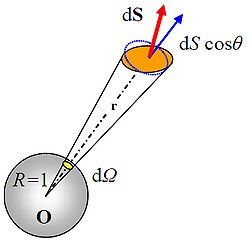
\includegraphics[scale=1]{angulosolido.jpg}
\end{figure}


Si llamamos a $\Omega$ el ángulo sólido, entendiendo elemento de ángulo sólido como $\D \Omega = \sin \theta \D \theta \D \phi$ podemos relacionar mediante la relación fundamental el número de partículas dispersadas en un elemento de ángulo sólido:

$$ \D N_{sc} = N_{inc} n_b \D \sigma $$

entonces está claro que la sección eficaz diferencial está relacionada con el elemento de ángulo sólido de tal manera que:

\begin{equation}
\D \sigma (\phi, \theta) = \frac{\D \sigma}{\D \Omega} (\phi, \theta) \D \Omega
\end{equation}

Donde el factor siguiente es la llamada \textbf{sección eficaz diferencial}:

\begin{equation}
\frac{\D \sigma}{\D \Omega} (\phi, \theta)
\end{equation}

Ahora vamos a relacionar la sección eficaz relacionar con el ángulo de scattering y el parámetro de impacto. Entonces si el ángulo sólido está centrado en el ángulo de dispersión $\theta$, y $b$ es el parámetro de impacto para el cual sale el proyectil con esa dispersión. Tenemos que para dicho ángulo de dispersión tendremos unas áreas que se relacionan como:

\begin{equation}
\D \sigma = 2 \pi b \D b
\end{equation}

tal y como se puede ver en la figura:


Además $\theta$ y $\Omega$ están relacionados ya que 

\end{document}

